%
% The first command in your LaTeX source must be the \documentclass command.
\documentclass[sigconf]{acmart}

%
% defining the \BibTeX command - from Oren Patashnik's original BibTeX documentation.
\def\BibTeX{{\rm B\kern-.05em{\sc i\kern-.025em b}\kern-.08emT\kern-.1667em\lower.7ex\hbox{E}\kern-.125emX}}


% Add additional
\usepackage{siunitx}
\usepackage{amssymb}
\usepackage{amsmath}
\usepackage{graphicx}
\usepackage{fancyvrb}
\usepackage{mathtools}
\usepackage[english]{babel}	
\usepackage{multirow}
\usepackage{enumitem} % for itemize labels
\usepackage{caption}
\usepackage{subcaption}
\usepackage{tikz}

% Rights management information. 
% This information is sent to you when you complete the rights form.
% These commands have SAMPLE values in them; it is your responsibility as an author to replace
% the commands and values with those provided to you when you complete the rights form.
%
% These commands are for a PROCEEDINGS abstract or paper.
\copyrightyear{2019}
\acmYear{2019}
\setcopyright{acmlicensed}
\acmConference[PASC '19]{PASC '19: The Platform for Advanced Scientific Computing Conference}{June 12--14, 2019}{Zurich, Switzerland}
%\acmBooktitle{Woodstock '18: ACM Symposium on Neural Gaze Detection, June 03--05, 2018, Woodstock, NY}
%\acmPrice{15.00}
%\acmDOI{10.1145/1122445.1122456}
%\acmISBN{978-1-4503-9999-9/18/06}

%
% These commands are for a JOURNAL article.
%\setcopyright{acmcopyright}
%\acmJournal{TOG}
%\acmYear{2018}\acmVolume{37}\acmNumber{4}\acmArticle{111}\acmMonth{8}
%\acmDOI{10.1145/1122445.1122456}

%
% Submission ID. 
% Use this when submitting an article to a sponsored event. You'll receive a unique submission ID from the organizers
% of the event, and this ID should be used as the parameter to this command.
%\acmSubmissionID{123-A56-BU3}

%
% The majority of ACM publications use numbered citations and references. If you are preparing content for an event
% sponsored by ACM SIGGRAPH, you must use the "author year" style of citations and references. Uncommenting
% the next command will enable that style.
%\citestyle{acmauthoryear}

%
% end of the preamble, start of the body of the document source.
\begin{document}

%
% The "title" command has an optional parameter, allowing the author to define a "short title" to be used in page headers.
\title{The Impact of Noise on Krylov Method Performance}


\iffalse
%
% The "author" command and its associated commands are used to define the authors and their affiliations.
% Of note is the shared affiliation of the first two authors, and the "authornote" and "authornotemark" commands
% used to denote shared contribution to the research.
\author{Hannah Morgan}
\email{hmorgan@anl.gov}
\affiliation{
  \institution{Mathematics and Computer Science, Argonne National Laboratory}
  \city{Argonne}
  \state{Illinois}
}

\author{Patrick Sanan}
\affiliation{
  \institution{Institute of Geophysics, ETH Zurich}
  \city{Zurich}
  \country{Switzerland}
  }

\author{Matthew Knepley}
\affiliation{
  \institution{Computer Science in Engineering, University of Buffalo}
  \city{Buffalo}
  \state{New York}
  \country{USA}
}

\author{Richard Mills}
\affiliation{
   \institution{Mathematics and Computer Science, Argonne National Laboratory}
  \city{Argonne}
  \state{Illinois}
  }
 
%
% By default, the full list of authors will be used in the page headers. Often, this list is too long, and will overlap
% other information printed in the page headers. This command allows the author to define a more concise list
% of authors' names for this purpose.
\renewcommand{\shortauthors}{Morgan, et al.}
\fi

%
% The abstract is a short summary of the work to be presented in the article.
\begin{abstract}
In this work, we develop a performance model and study the impact of 
operating system, machine variance, and other factors on Krylov and pipelined Krylov method execution.
We perform repeated runs and collect fine-grained data that 
 show the influence of variability on Krylov and pipelined Krylov methods.
To succinctly describe the execution performance, we 
 employ stochastic models based on the distribution of iteration times of each method.
 We test the models with collected data and suggest ways to improve and expand them in order to make a priori performance estimates.
\end{abstract}



%
% The code below is generated by the tool at http://dl.acm.org/ccs.cfm.
% Please copy and paste the code instead of the example below.
%
\begin{CCSXML}
<ccs2012>
<concept>
<concept_id>10002950.10003705.10011686</concept_id>
<concept_desc>Mathematics of computing~Mathematical software performance</concept_desc>
<concept_significance>500</concept_significance>
</concept>
<concept>
<concept_id>10002950.10003705.10003707</concept_id>
<concept_desc>Mathematics of computing~Solvers</concept_desc>
<concept_significance>300</concept_significance>
</concept>
<concept>
<concept_id>10010147.10010148.10010149.10010158</concept_id>
<concept_desc>Computing methodologies~Linear algebra algorithms</concept_desc>
<concept_significance>100</concept_significance>
</concept>
</ccs2012>
\end{CCSXML}

\ccsdesc[500]{Mathematics of computing~Mathematical software performance}
\ccsdesc[300]{Mathematics of computing~Solvers}
\ccsdesc[100]{Computing methodologies~Linear algebra algorithms}

%
% Keywords. The author(s) should pick words that accurately describe the work being
% presented. Separate the keywords with commas.
\keywords{Krylov, pipelining, noise, performance model, GMRES, PGMRES}

\maketitle

\section{Introduction}

% one page long-ish

Large-scale simulations often use Krylov methods \cite{saad96iterative,VanDerVorst2003} to solve sparse systems of equations in high performance computing (HPC) environments. 
As we move to more massively parallel computing the latency cost for global communication has skyrocketed \cite{HPCChallenge}, degrading the performance of Krylov methods because of the reduction operations used in each iteration.
To mitigate the latency associated with global communication, algebraically equivalent pipelined versions of Krylov methods have been introduced 
\cite{Chronopoulos_Gear_1989, GhyselsAshbyMeerbergenVanroose2013, GhyselsVanroose2014, StrzodkaGoddeke06, Sturler_Vorst_1995, JacquesNicolasVollaire12}. 
Pipelined methods rearrange computations so that it is possible to hide some of the cost of global communication with local computation. 

The increasing complexity of HPC computing environments has introduced many sources of run-to-run variability at different levels of HPC systems. 
For example, operating systems can interrupt processors at any time for its activities, causing detours in computations and degrading performance \cite{hoefler2010characterizing, FerreiraBridgesBrightwell08}.
Inter-job contention for shared resources such as network bandwidth, routers, and links is another source of variability that can affect application performance \cite{parker2017early, chunduri2017run}. 

Highly synchronous applications such as those that use Krylov methods are vulnerable to performance degradation induced by variability at different machine levels. 
Because each iteration is performed in lockstep, an operating system interrupt that delays a single processor can cause others to be delayed as well.
The variable amount of bandwidth available between iterations and runs can degrade Krylov methods because of the use of vector norms and orthogonalizations.
It is important to understand and characterize the performance of applications in order to evaluate HPC systems and algorithms. 
However, developing coherent performance models is difficult in the presence of variability \cite{beckman2006influence, HoeflerLumsdaineRehm07} particularly between systems. 

Employing stochastic performance models for algorithms that run on HPC systems could reflect a more realistic computing scenario since many detours and sources of variability are unpredictable.
Some work has been done using stochastic models to predict performance in HPC environments. 
For example, \cite{agarwal2005impact} studied the impact of different noise distributions on a single collective operation and \cite{seelam2010extreme} modeled operating system 
 ``jitter" as random variables in order to compute computational slowdown in the 
  presence of noise.
A stochastic performance model was introduced in \cite{morgan2016krylov} that described the performance of Krylov and pipelined Krylov methods in the presence of noise using random variables to model iteration times. 

In this work, we are interested in characterizing the performance of Krylov and pipelined Krylov methods on HPC systems in the presence of variability using experimental data and refining the performance model introduced in \cite{morgan2016krylov}.
We detail the results of experiments performed at the Argonne Leadership Computing Facility (ALCF) and the Swiss National Supercomputing Center and find that, using these results, our stochastic performance models can accurately describe runtimes and suggest a way to perform a priori estimates.

This paper is organized into several sections. Section \ref{sec:model-review} reviews the performance models introduced in \cite{morgan2016krylov} for Kylov and pipelined Krylov methods in the presence of system noise. In Section \ref{sec:experimental-results} we examine the results from runs of Krylov and pipelined Krylov methods and refine the performance models in Section \ref{sec:updated-model} based on insights from the experimental data.
In Section \ref{sec:performance-model} we employ our stochastic performance models and show that the updated model is in close agreement with reality.  In Sections \ref{sec:performance-estimates} and \ref{sec:more-experiments} we present more experimental data and suggest ways to perform a priori performance estimates.  Finally, we conclude our work in Section \ref{sec:conclusion}. 

\section{Stochastic model review} \label{sec:model-review}

A Krylov method is modeled as a set of $P$ processes repeatedly performing local computation and global communication. Because of the synchronizations in each of iteration, the processors perform in lockstep so that the total time for each iteration is the time given by the slowest processor. Let $p$ index the $P$ processors and $k$ index the $K$ iterations. Then, the total time $T$ for a Krylov method is modeled as
\begin{equation}
T = \sum_k \max_p T^k_p,
\end{equation}
where $T^k_p$ is the time for iteration $k$ on process $p$. Since this work can be interrupted by operating system noise interference, the iteration times $T^k_p$ might fluctuate over steps and processors. To model this nondeterministic behavior, we let the iterates be random variables and ask for the expected total runtime
\begin{equation}
E[T] = \sum_k E[ \max_p \mathcal{T}^k_p]. \label{eq:krylov-expression}
\end{equation}
If the iterates $\mathcal{T}^k_p$ are identical and independent of processor ($p$) and stationary in time ($k$), then we can compute the expected runtime of a Krylov method using the integral expression 
\begin{equation}
E[T] =  K P \int ^{\infty}_{-\infty} x F(x)^{P-1} f(x) dx \label{eq:krylov-model},
\end{equation}
where the random variables $\mathcal{T}^k_p$ are drawn from a distribution with probability density function (pdf) $f(x)$ and cumulative distribution function (cdf) $F(x)$. 

Similarly, we model a pipelined Krylov method as a set of $P$ communicating processors. Pipelined methods employ split-phase collectives that do not require global synchronizations. Rather, the collective operation is first initialized, say with  ${\texttt{MPI\_Iallreduce()}}$, and later finalized with ${\texttt{MPI\_Wait()}}$ so that useful work can continue between initialization and finalization. 
Provided no processor falls too far behind, the total time for a pipelined method $T'$ is the time for the slowest processor to perform all the given work 
\begin{equation}
T' = \max_p \sum_k T^k_p.
\end{equation}
Because of detours, we do not expect the iteration times to be constant. Again, we ask for the expected total run time
\begin{equation}
E[T'] = E\left[\max_p \sum_k \mathcal{T}^k_p\right], \label{eq:pipeline-expression}
\end{equation}
letting the iterates be random variables drawn from a distribution. 
If the iterates $\mathcal{T}^k_p$ are identically distributed with finite mean and variance, independent of process ($p$) and stationary in time ($k$), then, in the limit of large $K$, $\tfrac{1}{K}\sum_k\mathcal{T}^k_p \rightarrow \mu$ where $\mu$ is the mean of the underlying iteration time distribution with pdf $f(x)$ and cdf $F(x)$. So we have an expression to compute the expected total time for a pipelined method
\begin{equation}
E[T'] \rightarrow K\mu. \label{eq:pipeline-model}
\end{equation}

For a more thorough explanation of the arguments presented in this section, see \cite{morgan2016krylov}.
In the next section we present fine-grained data collected from runs of Krylov and pipelined Krylov methods. This gives us insight into how detours affect these simulations, which assumptions above are realistic, and how the models might be refined. 

\section{Experimental results} \label{sec:experimental-results}

Here we present the results from a set of experiments run on the Cray XC40 Theta at the Argonne Leadership Computing Facility. 
Theta contains Xeon Phi Knights Landing (KNL) compute nodes \cite{sodani2015knights} with 64 CPU processors per node connected by a Cray Aries interconnect with dragonfly topology \cite{alverson2012cray}.
We use the Portable, Extensible Toolkit for Scientific Computation (PETSc) \cite{petsc-user-ref, petsc-web-page} software package to simulate the solution to problems with varying characteristics such as sparsity pattern. 
One MPI rank per core is used throughout and we boot the nodes in quadrant clustering mode with flat memory mode. 
We collect iteration times $\mathcal{T}^k_p$ by inserting calls to ${\texttt{MPI\_Wtime()}}$ at the beginning and end of each Krylov cycle in PETSc's scalable linear equation solvers (KSP) component's GMRES (generalized minimal residual method) and PGMRES (pipelined GMRES) methods \cite[Alg. 4]{GhyselsAshbyMeerbergenVanroose2013}. 
Since changes and upgrades to HPC machines can affect performance, we note that experiments presented in this paper were performed in autumn 2018. 

%Select data can be found in the open Bitbucket repository \cite{morgan2017theta}.

\subsection{One-dimensional Laplacian} \label{sec:ex23}
PETSc KSP tutorial ex23\footnote{\texttt{/src/ksp/ksp/examples/tutorials/ex23.c} in PETSc 3.10} is a one-dimensional discretization of the Laplacian, resulting in a simple tridiagonal system. 
We run ex23 with GMRES and PGMRES on 8192 processors with $10^6$ unknowns and a Jacobi preconditioner. 
Throughout these simulations we force 5000 iterations of the Krylov method.


\begin{figure}[t]
\centering
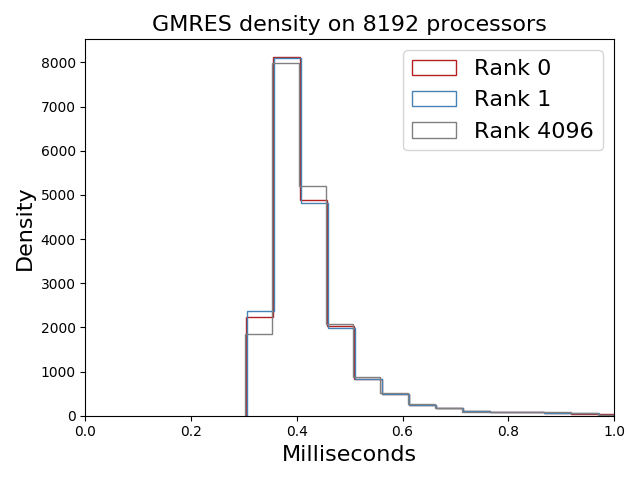
\includegraphics[width=6cm]{../plots/GMRES_ex23_8192_1000000_identical_in_p.png}
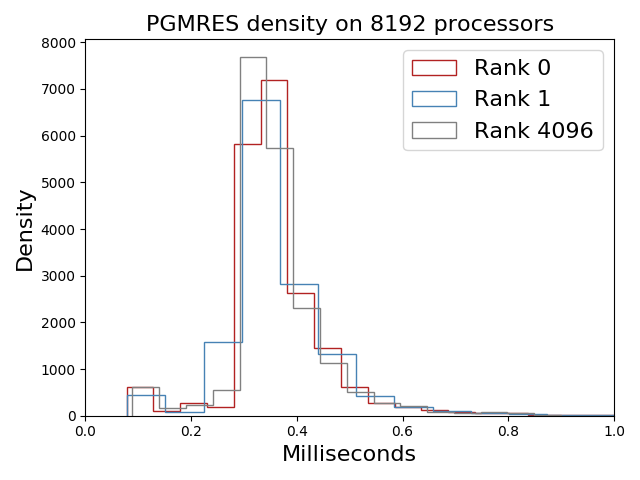
\includegraphics[width=6cm]{../plots/PGMRES_ex23_8192_1000000_identical_in_p.png}
\caption{Distribution of iterates $\mathcal{T}^k_p$ for fixed processors.} \label{fig:ex23-identical}
\end{figure}



The stochastic model expressions \eqref{eq:krylov-model} and \eqref{eq:pipeline-model} place assumptions on the iterates $\mathcal{T}^k_p$. We check them here to examine the actual performance of the algorithms and to justify use of the models. 
In Figure \ref{fig:ex23-identical} we graph the distribution of the iterates for select processors identified by their MPI ranks. The distributions look similar between ranks, implying that the iterations might be identical with respect to process. We make use of the two sample Kolmogorov-Smirnov test to check whether two samples (e.g. iterations from rank 0 and rank 1) are drawn from the same underlying distribution. The Kolmogorov-Smirnov test calculates the distance between the empirical distributions of two samples with empirical distribution functions $F_1$ of size $n$ and $F_2$ of size $m$ with
$$ D = \sup_x |F_1(x) - F_2(x)|. $$
We reject the hypothesis that the samples come from the same distribution with significance level $\alpha$ if 
$$D > c(\alpha)\sqrt{\frac{n + m}{nm}}$$
where $c(\alpha)$ is a tabulated value. 
For GMRES, $n = m = 5000$ and $n = m = 5334$ for PGMRES. We use significance level $\alpha = 0.05$ and SciPy's ${\texttt{stat.ks\_2samp}}$ function to calculate the test statistic $D$.  
We find that we do not reject that GMRES ranks 0 and 1 come from the same distribution with significance level $\alpha = 0.05$ since $D = 0.002 < 0.024$, the threshold. For PGMRES ranks 0 and 1, $D = 0.088 > 0.023$, so we reject the null hypothesis. 
On rank 1, we reject none of the $P-1$ pairs of GMRES ranks and reject $54.5\%$ of PGMRES pairs.
%Overall, we do not reject $x\%$ of the $\frac{P(P-1)}{2}$ pairs of GMRES ranks and $y\%$ of PGMRES ranks.

Because it is inefficient to orthogonalize against a very big basis, GMRES methods are typically implemented to restart after $R$ iterations. When a Krylov method restarts, the basis for the Krylov space is discarded and the current solution is used as the initial guess for the next cycle.
Since the PETSc default restart value is $30$ and each cycle of PGMRES uses two additional iterations to ``fill the pipeline," 5334 iterations are actually employed instead of 5000. Some of these are very quick and easily identifiable as the bump of very short iterations in Figure \ref{fig:ex23-identical} (right). 

\iffalse
\begin{figure}
\centering
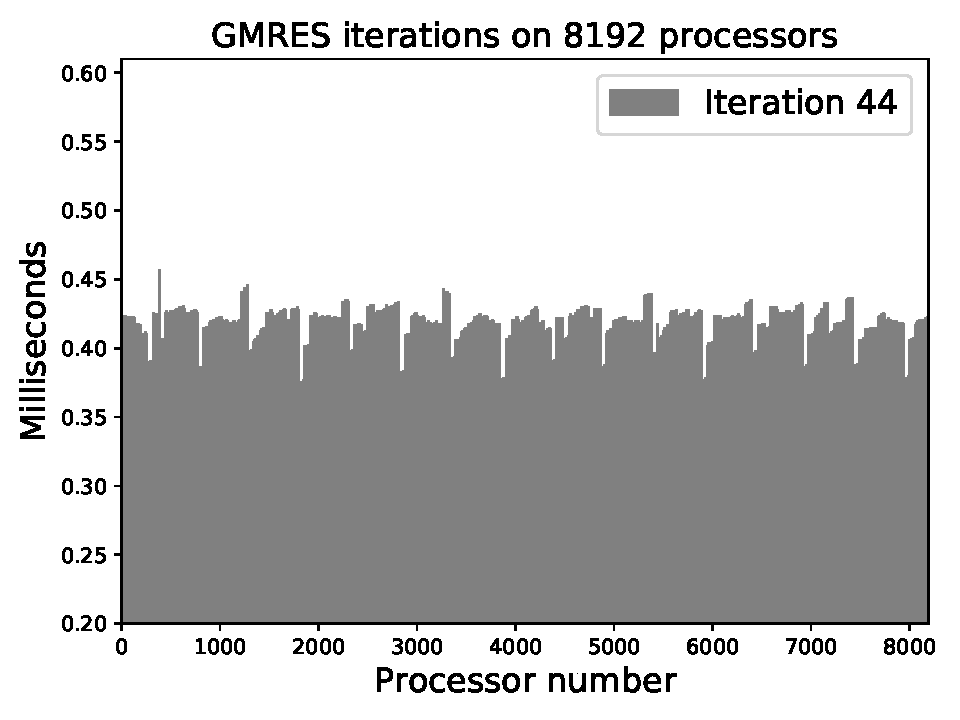
\includegraphics[width=6cm]{../plots/GMRES_ex23_8192_1000000_independent_in_p_44.pdf}
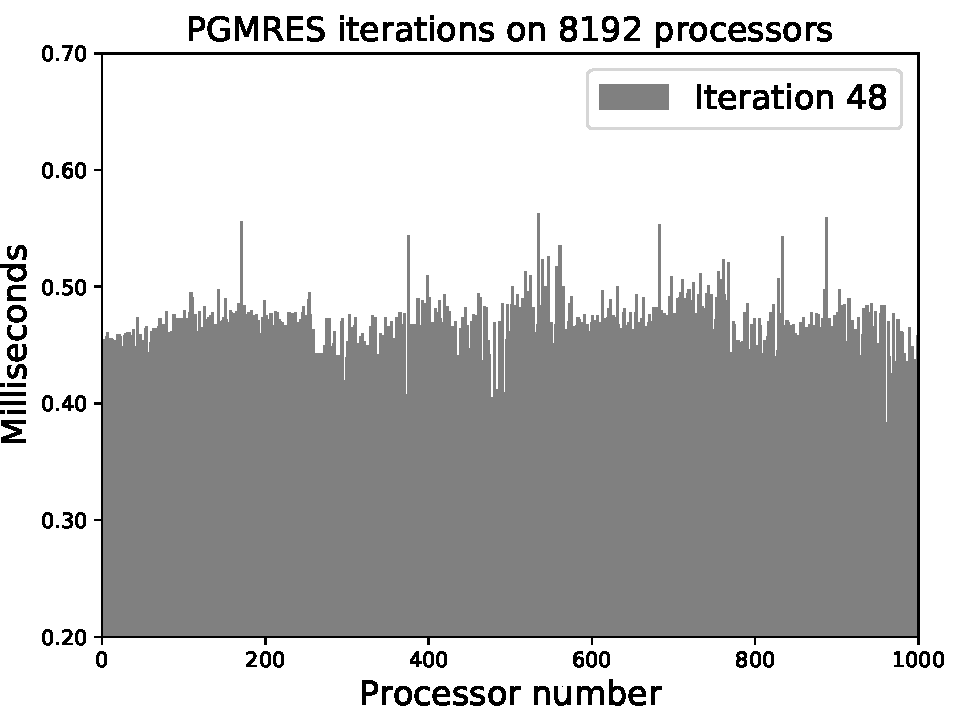
\includegraphics[width=6cm]{../plots/PGMRES_ex23_8192_1000000_independent_in_p_48.pdf}
\caption{Time for iterations $k=44$ (GMRES) and $k=48$ (PGMRES) on process $p$. }
 \label{fig:ex23-independent}
\end{figure}
\fi

\begin{figure}
 \centering
   \begin{tikzpicture}
     \node at (0, 0) {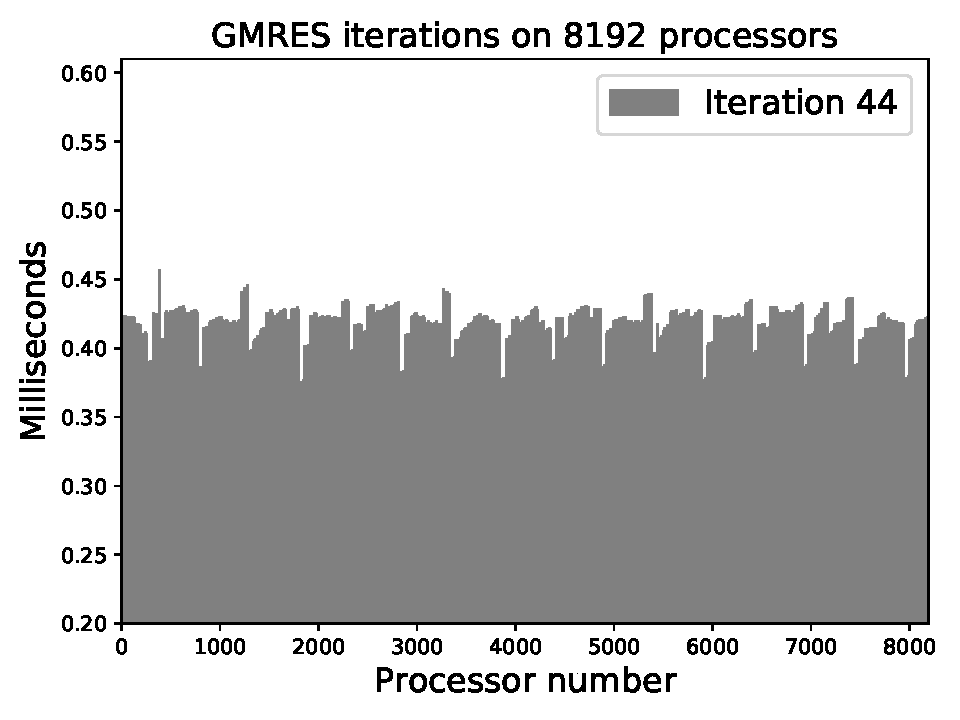
\includegraphics[width=6cm]{../plots/GMRES_ex23_8192_1000000_independent_in_p_44.pdf}};
     \node at (-1.15, -.8) {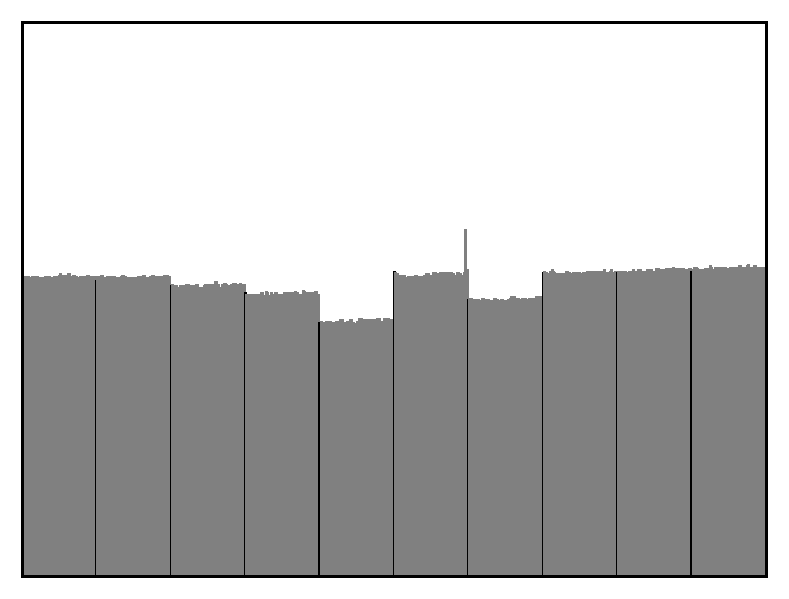
\includegraphics[width=2cm]{../plots/GMRES_ex23_8192_1000000_independent_in_p_inset_44_with_lines.pdf}};
  \end{tikzpicture}
     \begin{tikzpicture}
     \node at (0, 0) {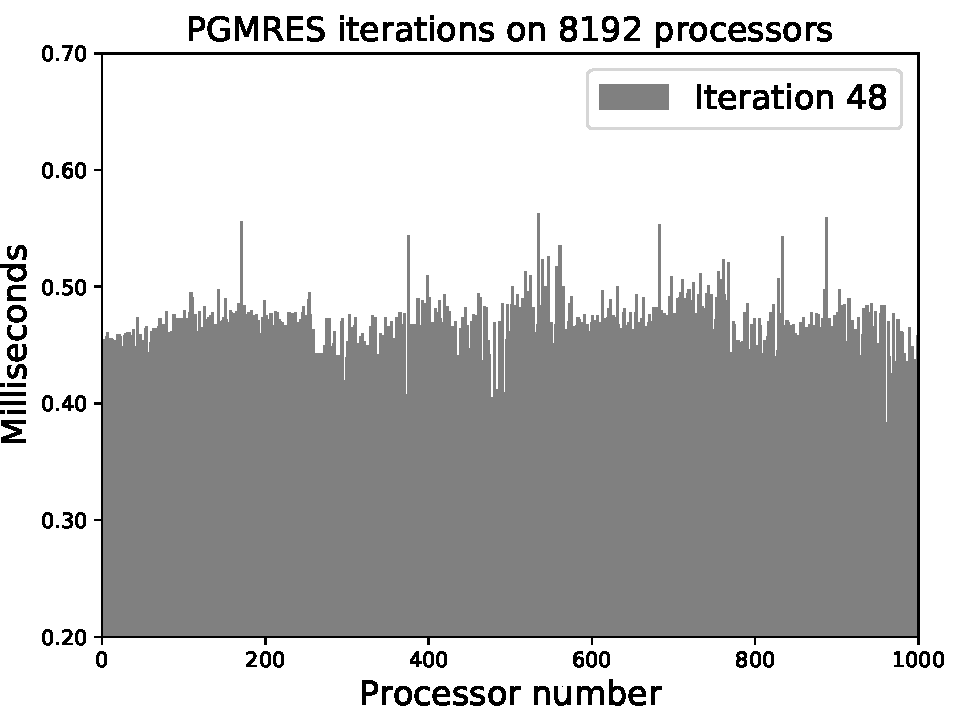
\includegraphics[width=6cm]{../plots/PGMRES_ex23_8192_1000000_independent_in_p_48.pdf}};
     \node at (-1.27, -.88) {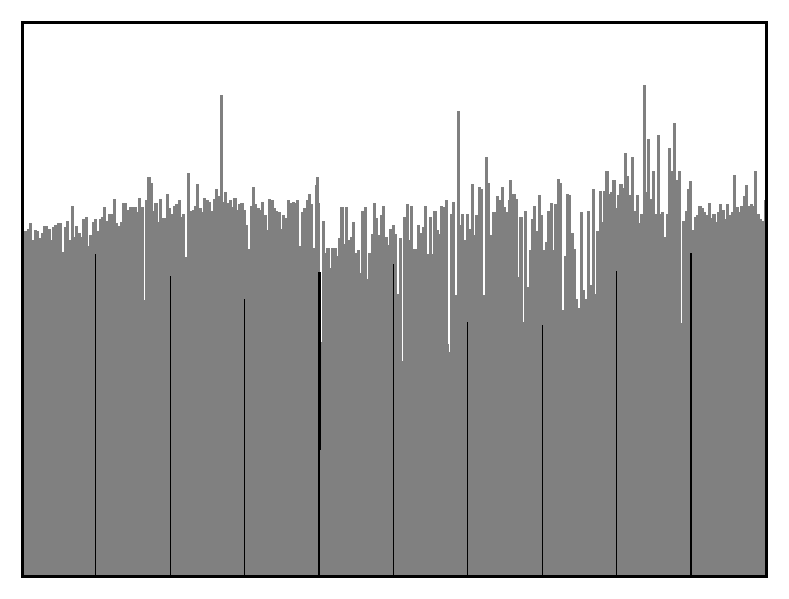
\includegraphics[width=2cm]{../plots/PGMRES_ex23_8192_1000000_independent_in_p_inset_48_with_lines.pdf}};
  \end{tikzpicture}
\caption{Time for iterations $k=44$ (GMRES) and $k=48$ (PGMRES) on process $p$ with inset showing the first 10 nodes. }
 \label{fig:ex23-independent}
\end{figure}


Figure \ref{fig:ex23-independent} shows the time for iterations $k=44$ (GMRES) and $k=48$ (PGMRES) on process $p$ in order of MPI rank. Iterates are drawn with grey bars and we include a inset graph that shows the iterations on the first ten nodes, delineated by black lines. 
GMRES iterates are nearly constant on a node; each KNL node of 64 processors is clearly visible in Figure \ref{fig:ex23-independent} (left, inset) so that the iterations are not truly independent in $p$ as we assumed above. The variance of iteration times on node 0 (with MPI ranks 0-63) is $6.3\cdot10^{-13}$. 
This could be due to the synchronizations in each iteration of GMRES, forcing processors on a node to perform in lockstep. 
There is also some periodic behavior over all the nodes.
Conversely, PGMRES iterations appear to contain more variability on a node ($1.4\cdot10^{-10}$ on the node with MPI ranks 0-63, three orders of magnitude greater than GMRES), but less between them. 

\begin{figure}[b]
\centering
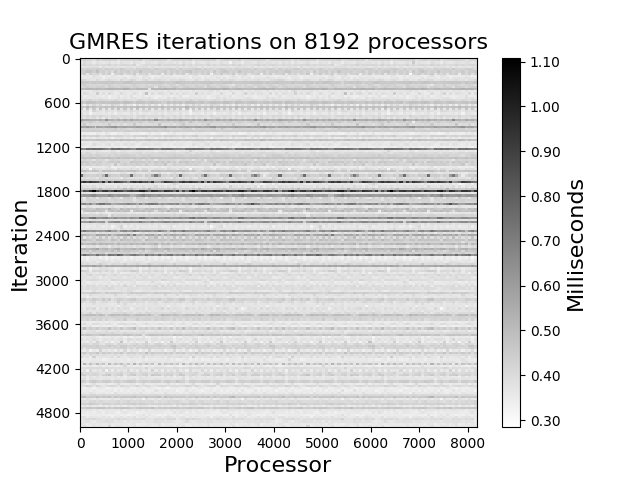
\includegraphics[width=6cm]{../plots/GMRES_ex23_8192_1000000__stationary_in_t_colormap.png}
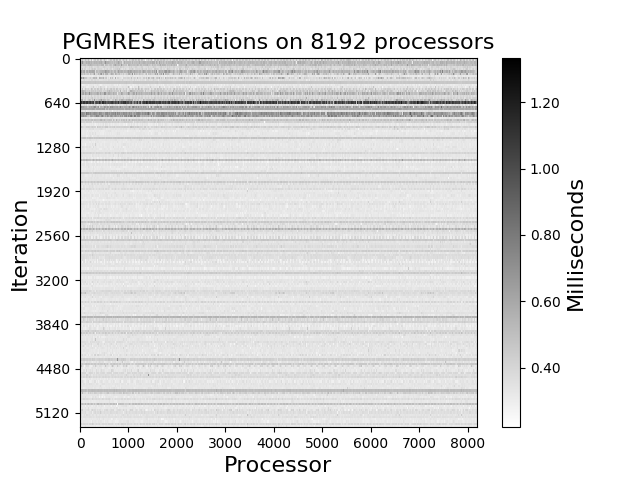
\includegraphics[width=6cm]{../plots/PGMRES_ex23_8192_1000000__stationary_in_t_colormap.png}
\caption{Colormap of iterates $\mathcal{T}_p^k$.} \label{fig:ex23-stationary}
\end{figure}




Figure \ref{fig:ex23-stationary} is a colormap of the iterates $\mathcal{T}_p^k$ for all iterations and all processors.
Graphed are the iterations that perform the ``average" amount of work during each GMRES cycle (GMRES iteration $14 \bmod 30$ and PGMRES $16 \bmod 32$) so that each iteration shown performs the same computation. 
Horizontal lines are highly visible, implying that processors perform similarly within a given iteration. 
The difference between different iterations is also clear so that the iterates seem to jump around in time without an obvious pattern.
There are some groups of iterations (GMRES iterations $k \approx 1700 - 2300$ or PGMRES $k \approx 640 - 740$) that overall take longer than other iterations. This could be explained by some longer operating system interruption.

The derivations in Section \ref{sec:model-review} made the simplifying assumption that the iterates were stationary in time so that the sum in \eqref{eq:krylov-expression} could become a product in \eqref{eq:krylov-model}. We account for this non-stationary behavior when we refine the performance model in Section \ref{sec:updated-model}.



\subsection{Blatter-Pattyn equations}
PETSc SNES tutorial ex48\footnote{\texttt{src/snes/examples/tutorials/ex48.c} in PETSc 3.10} solves the hydrostatic equations for ice sheet flow, where the ice uses a power-law rheology with Glen exponent 3. This generates a much denser system of equations with about 10 times more nonzeros per row than ex23. Again we choose our problem size so that there are $10^6$ unknowns, use a Jacobi preconditioner, and force 5000 iterates of the Krylov method. We stop after one nonlinear iteration. 

We repeat the analysis from Section \ref{sec:ex23} and find qualitatively similar results, shown in Figure \ref{fig:ex48}. Using the Kolmogorov-Smirnov test again we find that we do not reject the assumption that GMRES iterates from ranks 0 and 1 come from the same distribution since $D = 0.003 < 0.024$ and we reject that PGMRES iterates come from the same distribution since $D = 0.078 > 0.023$.
The iterates on a fixed process $p$ look like they could be from the same family of distributions with different parameters as those in the previous subsection. 

GMRES iterates again appear highly dependent on the node with node 0 variance $4.3\cdot10^{-13}$. The variance on PGMRES node 0 is $8.6\cdot10^{-10}$, larger than before, and there is more variation between PGMRES nodes which looks periodic. This could be explained by the communication induced by the matrix sparsity pattern. While certain nodes appear to take much longer, the colormap (bottom right) shows that overall processors perform similarly within an iteration. Again, the computation is  not stationary in time. 

\begin{figure}[t]
\centering
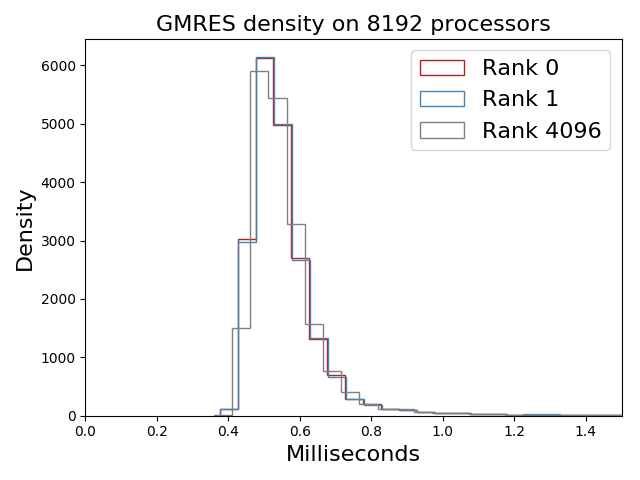
\includegraphics[width=4cm]{../plots/GMRES_ex48_8192_1000000_identical_in_p.png}
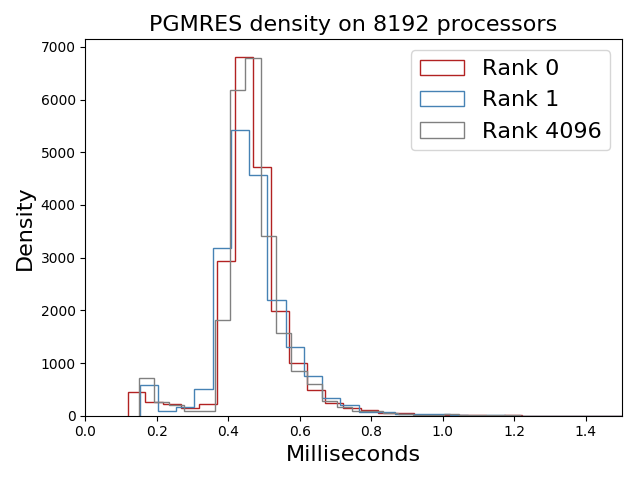
\includegraphics[width=4cm]{../plots/PGMRES_ex48_8192_1000000_identical_in_p.png} \\
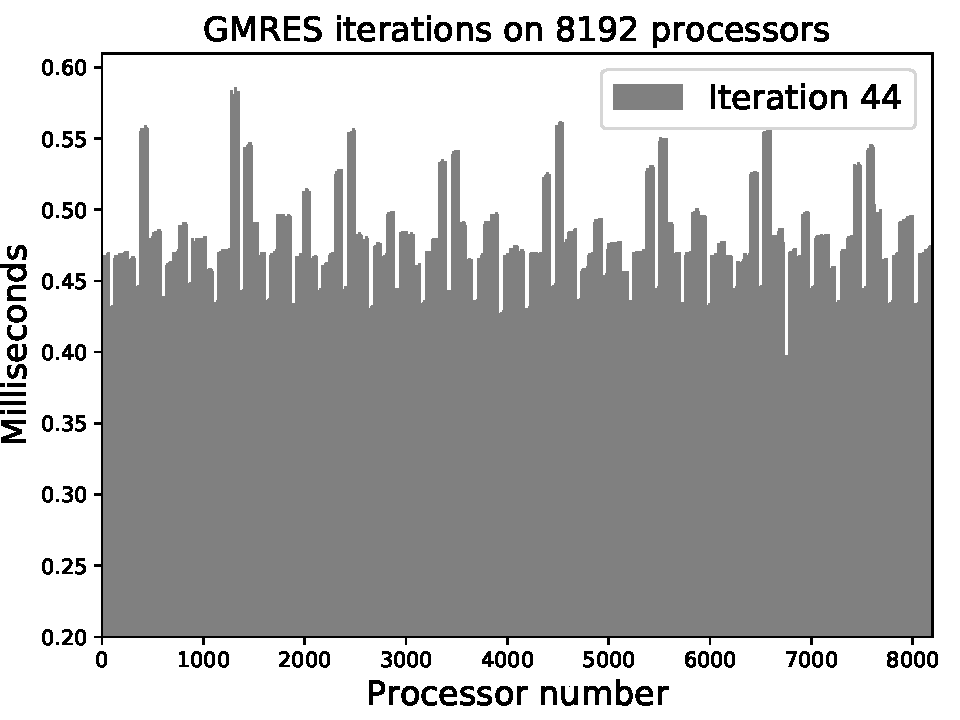
\includegraphics[width=4cm]{../plots/GMRES_ex48_8192_1000000_independent_in_p_44.pdf}
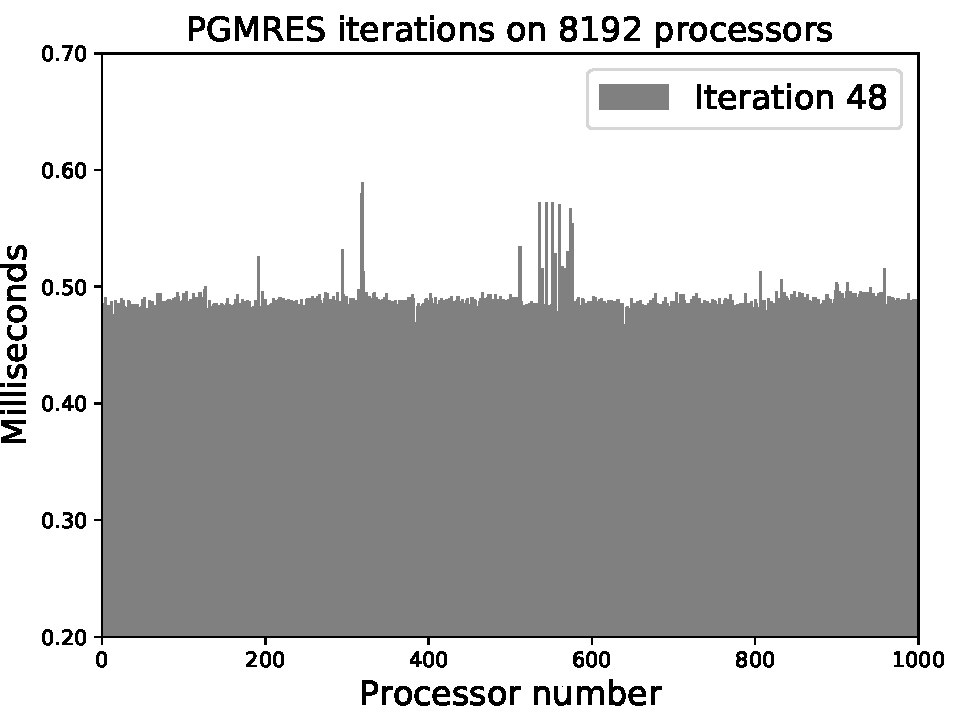
\includegraphics[width=4.3cm]{../plots/PGMRES_ex48_8192_1000000_independent_in_p_48.pdf} \\
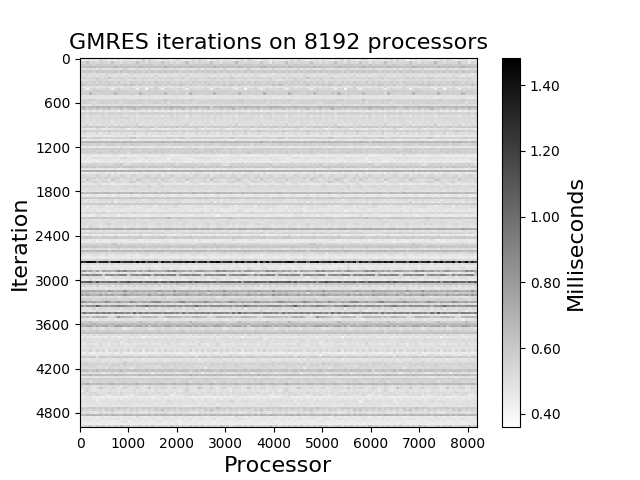
\includegraphics[width=4.3cm]{../plots/GMRES_ex48_8192_1000000_stationary_in_t_colormap.png} 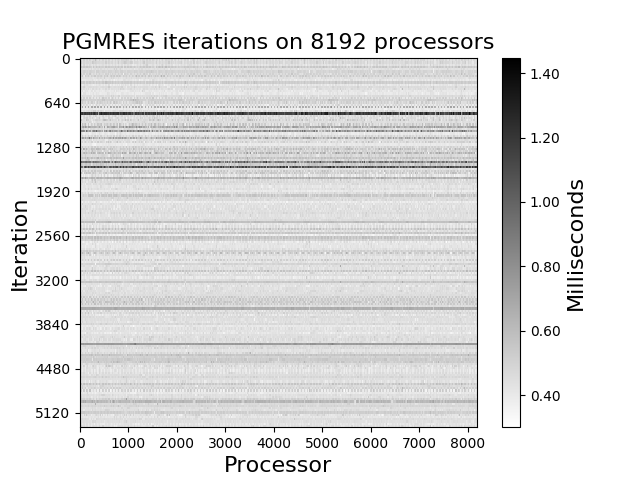
\includegraphics[width=4cm]{../plots/PGMRES_ex48_8192_1000000_stationary_in_t_colormap.png}
\caption{GMRES (left) and PGMRES (right) iterations for PETSc ex48.} \label{fig:ex48}
\end{figure}



\section{Non-stationary performance model} \label{sec:updated-model}

Based on the results from the last section, we move to a non-stationary performance model where the iterates $\mathcal{T}^k_p$ can fluctuate in time.
The expected total time for a Krylov method is still given by 
$$E[T] = \sum_k E[ \max_p \mathcal{T}^k_p]$$
but we relax the claim that the iterates are stationary in time. In iteration $k$, the random variables $\mathcal{T}^k_p$ are drawn from a distribution with cdf $F_k(x)$ and pdf $f_k(x)$, which can now fluctuate across steps.
Then the expected runtime of a Krylov method is given by 
\begin{equation}
\widehat{E}[T] =  \sum_k P \int ^{\infty}_{-\infty} x F_k(x)^{P-1} f_k(x) dx. \label{eq:updated-krylov-model},
\end{equation}
We call this the ``non-stationary" performance model and distinguish between $E[T]$ in \eqref{eq:krylov-model} and $\widehat{E}[T]$ here.


Similarly for a pipelined method, we use \eqref{eq:pipeline-expression} as before and drop the assumption that the iterates are stationary in time, so that
\begin{equation}
\widehat{E}[T'] \rightarrow  \sum_k \mu_k \label{eq:updated-pipelined-model},
\end{equation}
where $\mu_k$ is the mean of the underlying distribution in iteration $k$. 

The original Krylov model \eqref{eq:krylov-model} benefits from slight alteration as well. 
Since the iterates on each node are nearly constant, shown in Figure \eqref{fig:ex23-independent} (left) and Figure \ref{fig:ex48} (top middle), they are more suitably modeled by $\widehat{P} = P/64$  independent random variables than $P$ independent processors. We make use of this substitution in the next section but it does not seem to strongly affect \eqref{eq:updated-krylov-model}.


\section{Performance modeling} \label{sec:performance-model}

In this section, we will deploy our performance models and test them against collected data.

\subsection{Computing expected runtimes} \label{sec:computing-runtimes}

The expressions for $E[T]$ and $E[T']$ say that the iterates come from some underlying  distribution with pdf $f(x)$, cdf $F(x)$, and mean $\mu$. 
We will use ``bulk statistics" with these performance models, taking all iterations for all processors in aggregate, for the underlying distribution and to characterize the iteration times and machine variation. 

\begin{figure}[b]
\centering
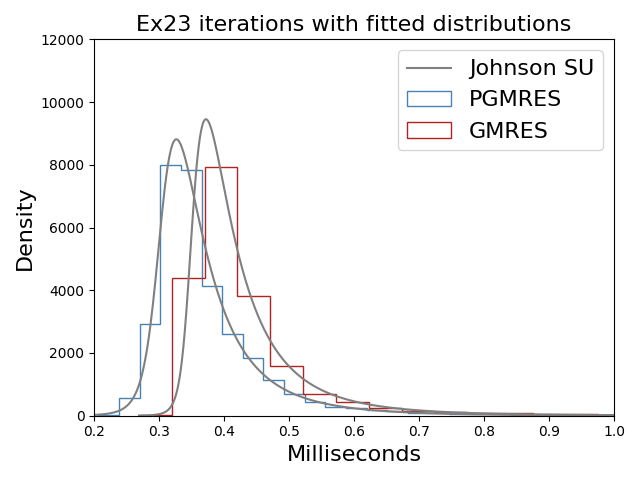
\includegraphics[width=6cm]{../plots/GMRES_PGMRES_ex23_8192_1000000_bulk_stats_with_johnsonsu.png}
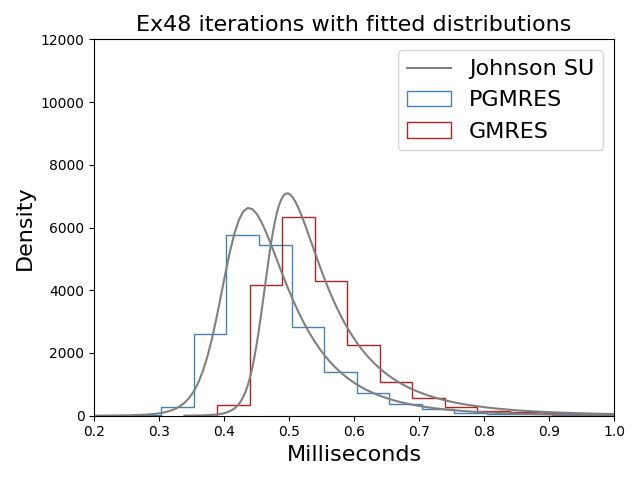
\includegraphics[width=6cm]{../plots/GMRES_PGMRES_ex48_8192_1000000_bulk_stats_with_johnsonsu.png} 
\caption{GMRES and PGMRES bulk statistics with fitted distributions for PETSc ex23 (left) and ex48 (right).} \label{fig:bulk-fitted}
\end{figure}

To find the functions $f(x)$ and $F(x)$ and mean $\mu$, we use Scipy's ${\texttt{stats}}$ package to fit various analytical distributions to our collected data. For a given continuous distribution and data, the ${\texttt{fit}}$ function returns the maximum likelihood estimation for the shape, location, and scale parameters by maximizing a log-likelihood function.  
We choose distributions which minimize the sum of squared error between the data and the fit distribution.
For the pipelined methods, we disregard the two iterations in each cycle that ``fill the pipeline" to avoid distribution fitting complications.




Using these well-fitting distributions, we can calculate $E[T]$ and $E[T']$ and compare the expected results to the actual \texttt{KSPSolve times} (the time spent inside the Krylov solver) provided by PETSc's ${\texttt{-log\_view}}$ option. 
For integration in \eqref{eq:krylov-model} we use Python's ${\texttt{quad}}$ function and integrate over the bounds of the data.

To employ the updated models $\widehat{E}[T]$ and $\widehat{E}[T']$, we again perform distribution fitting using ${\texttt{scipy}}$, this time for each iteration to find  $f_k(x)$, $F_k(x)$, and mean $\mu_k$.
We claim that the runtimes $\mathcal{T}^k_p$ for each iteration $k$ are from the same family with possibly different parameters. 
Not all iterations resemble the same distribution family, so we use a uniform distribution to model the iterations, shown fitted to GMRES and PGMRES iterations in Figure \ref{fig:iterations-with-fitted-uniform}. 
The distribution parameters vary by iteration.
In \eqref{eq:updated-krylov-model}, integration is performed in each iteration again using ${\texttt{quad}}$ and the calculated expected total times are compared to the \texttt{KSPSolve} time.

Analytical expressions have been used \cite{seelam2010extreme} to bound the maximum of a set of random variables using the sample mean $\mu_X$ and standard deviation $\sigma_X$.  Cramer \cite{cramer2016mathematical, david2004order} bound the maximum of $N$ identical and independent random variables  with
\begin{equation}
E[X_{\max{(N)}}] \leq \mu_X + \frac{\sigma_X (N-1)}{\sqrt{2N-1}}
\end{equation}
and Bertsimas \cite{bertsimas2006tight} bound the maximum of $N$ identical, but not independent random variables by
\begin{equation}
E[X_{\max{(N)}}] \leq \mu_X + \sigma_X \sqrt{N-1}.
\end{equation}
We will use these to compare with our Krylov performance models.

\subsection{Results}

Distribution fitting alone gives some insight into algorithm execution. 
In Figure \ref{fig:bulk-fitted}, we show bulk data from Section \ref{sec:experimental-results} with the Johnson SU distribution. Note that there were some other well-fitting distributions, including Non-central Student's T.
The bulk data show that in a given method, the iterates $\mathcal{T}^k_p$ are mostly clustered and fairly quick with a fewer, longer, giving the distribution a small tail.
In general, PGMRES runtimes were faster than GMRES, consistent with faster overall execution in these examples. Ex48 runtimes are shifted to the right of ex23 and more spread out, implying longer iterations with more variation. 


Results for the data presented in Section \ref{sec:experimental-results} are shown in Table \ref{tab:performance-model} for PETSc ex23 and ex48.
We see that the original model for the expected time of a Krylov method $E[T]$  overestimates the actual runtimes and is not a particularly good estimate, nor is any bulk distribution best in all cases.  On the other hand, the updated Krylov model $\widehat{E}[T]$ is a big improvement for traditional Krylov methods and makes a reasonable prediction. The analytical bounds are very loose and not particularly helpful.
$E[T']$ and $\widehat{E}[T']$ are both good estimates for the pipelined method, suggesting that modeling a method without explicit synchronization is more flexible. 
In one case, the non-stationary model $\widehat{E}[T']$ is not as good a predictor for PGMRES, but it is more representative of the actual process. 
The results show that when we have available iteration data, the updated performance models \eqref{eq:updated-krylov-model} and \eqref{eq:updated-pipelined-model} are good performance predictors and we will use them from here on. 

\begin{table*}[t]
\caption{Performance model results and bounds for ex23 and ex48 with well-fitting distributions.}
\begin{center}
\begin{tabular}{| l l l l l  l l |} \hline
 ex23 & KSPSolve & $E_{\text {JohnSU}}\left[T\right]$ & $E_{\text {NCT}}\left[T\right]$ & $\widehat{E}_{\text {Unif}}\left[T\right]$  & Cramer bound & Bertsimas bound \\
 GMRES & 2.217 & 4.831 & 4.365   & 2.432  & 6.35 & 8.102 \\
 PGMRES & 2.006 & 1.865 & 1.868 & 1.857 & &  \\ \hline
 ex48 &  &  &  &  & & \\
 GMRES & 2.943 & 5.716 & 10.88  & 3.189 & 20.59  & 27.99 \\
 PGMRES & 2.656 & 2.413 & 2.413 & 2.455   & & \\
\hline  % Please only put a hline at the end of the table
\end{tabular} \label{tab:performance-model}
\end{center}
\end{table*}

\iffalse
The original models use bulk statistics and an underlying distribution to describe the iterations in aggregate. We found Johnson SU to be a good fit with our data. 

We can use these parameters to reason about different Krylov runs.
For example, the location and scale parameters for both GMRES and PGMRES are smaller in ex23 than those in ex48, meaning that the distributions in ex23 are shifted to the left and more compressed than those fitted to the data of ex48.
\fi


\section{Predicting runtimes}\label{sec:performance-estimates}

In the previous section, we showed that our performance models $\widehat{E}[T]$ and $\widehat{E}[T']$ can reasonably predict execution time when we have the time for iteration $k$ on process $p$ for all $k$ and $p$. 

\begin{figure}[b]
\centering
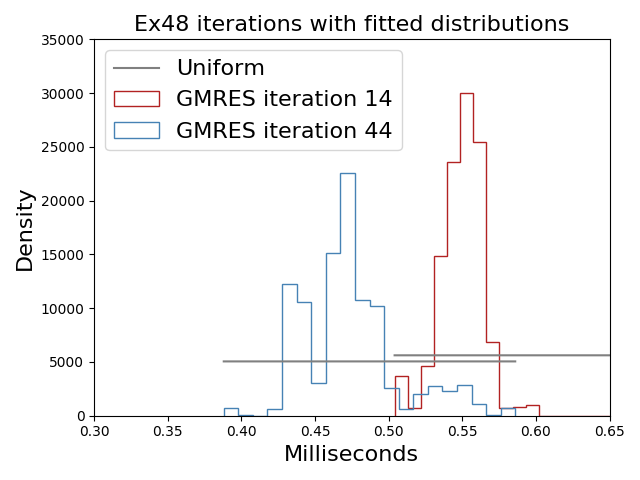
\includegraphics[width=4cm]{../plots/GMRES_ex48_8192_1000000_stationary_in_t_with_uniform_14_44.png}
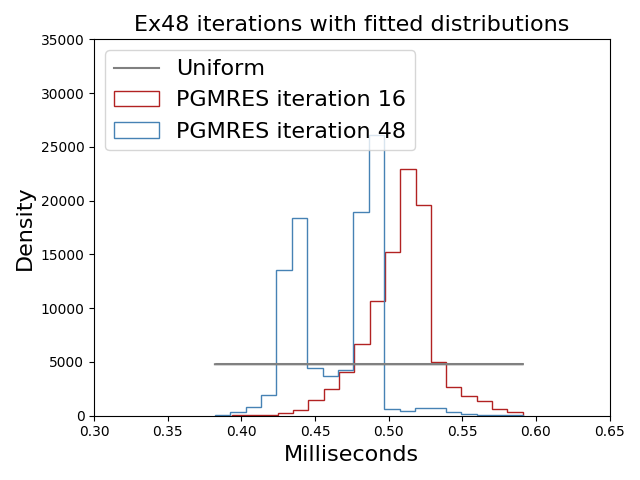
\includegraphics[width=4cm]{../plots/PGMRES_ex48_8192_1000000_stationary_in_t_with_uniform_16_48.png}
\caption{GMRES  iterations $k = 14, 44$ and PGMRES $k = 16, 48$ iterations  with fitted uniform distributions.} \label{fig:iterations-with-fitted-uniform}
\end{figure}

Bulk statistics appear to be enough to succinctly describe the performance of a pipelined method, they are not a sufficient way to describe a traditional Krylov method. Instead, we used non-stationary uniform distributions to model each iteration, shown in Figure \ref{fig:iterations-with-fitted-uniform}.
Here we see how non-stationary the iterations actually are, in this case they are almost non-overlapping, and how the parameters change over time. 
That is, for each iteration $k$, the random variables $\mathcal{T}_p^k$ are modeled as following a uniform distribution with pdf $f_k$ and cdf $F_k$ given by
\begin{equation} \label{eq:uniform}
f_k(x) = \frac{1}{b_k - a_k}, \quad F_k(x) = \frac{x-a_k}{b_k-a_k}.
\end{equation}
The uniform distribution can be described with two parameters: the minimum $a_k$ and the span $s_k = b_k - a_k$. We model a Krylov method with $K$ uniform distributions
where in each iteration the uniform parameters $a_k$ and $s_k$ are random variables themselves drawn from some distribution. 
Figure \ref{fig:uniform-params-fitted} show histograms of the uniform parameters from  PETSc ex48 using GMRES and PGMRES with fitted Johnson SU distribution.
Johnson SU, a transformation of the normal distribution, is described by two shape parameters $a$ and $b$ and location and scale parameters ${\texttt{loc}}$ and ${\texttt{scale}}$ in Scipy.  

\begin{figure}[t]
\centering
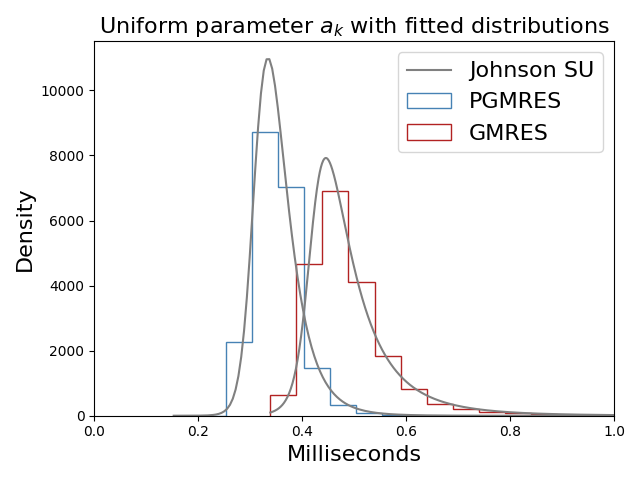
\includegraphics[width=6cm]{../plots/GMRES_PGMRES_ex48_8192_1000000_uniform_a_k_with_johnsonsu.png}
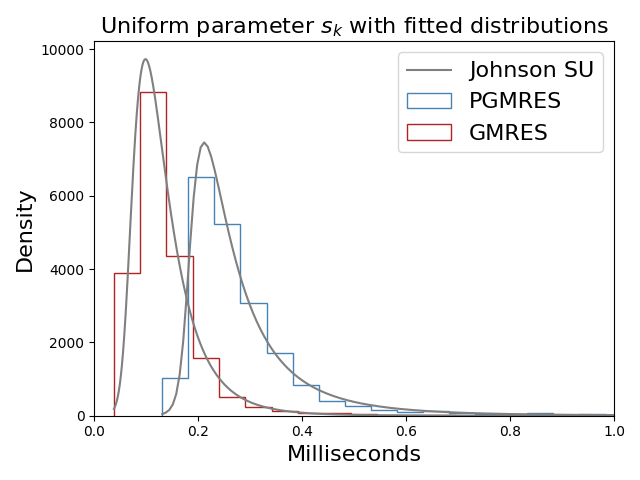
\includegraphics[width=6cm]{../plots/GMRES_PGMRES_ex48_8192_1000000_uniform_s_k_with_johnsonsu.png} 
\caption{Uniform parameters $a_k$ and $s_k$ from PETSc ex48 with fitted distributions.} \label{fig:uniform-params-fitted}
\end{figure}

The location and scale parameters shift the distribution left and right (${\texttt{loc}}$) and stretch and shrink horizontally (${\texttt{scale}}$) so that standardizing the distribution with ${\texttt{loc}} = 0$ and ${\texttt{scale}} = 1$ involves the transformation $y = (x - {\texttt{loc}})/{\texttt{scale}}$.
Table \ref{tab:distribution-params} shows Johnson SU parameters for the  uniform distribution parameters from Figure \ref{fig:uniform-params-fitted} and PETSc ex23. In general, they show that, in a given iteration, the fastest processor is generally faster in a PGMRES run, but the runtimes are more spread out. All Johnson SU distributions are shaped such that they lean left with a tail, some longer than others.

To simulate a Krylov computation, we assume that each iteration time $\mathcal{T}_p^k$ is uniformly distributed with parameters $a_k$ and $s_k$ in iteration $k$
$$\mathcal{T}_p^k \sim \text{Uniform}(a_k, s_k).$$ 
We further assume that the parameters $a_k$ and $s_k$ are themselves random variables drawn from a Johnson SU distribution with parameters $a$, $b$, $\texttt{loc}$, and $\texttt{scale}$.

We draw random variables $a_k$ and $s_k$  using Scipy's $\texttt{rvs}$ function, which generates random variates from a distribution and compute the expected time for iteration $k$, $\widehat{E}[T_k]$, given by 
\begin{equation}
\widehat{E}[T_k] =  \widehat{P} \int ^{\infty}_{-\infty} x F_k(x)^{\widehat{P}-1} f_k(x) dx.
\end{equation}
Repeating for $K$ iterations, we get $\widehat{E}[T]$. 
We simulate a pipelined Krylov computation in the same way, pulling random variables $a_k$ and $s_k$ and computing 
\begin{equation}
\widehat{E}[T'_k] =  \mu_k
\end{equation}
where $\mu_k$ is the mean of $\text{Uniform}(a_k, s_k)$. 
Table \ref{tab:simulated-runtimes} shows the results of this simulation using the Johnson SU parameters from Table \ref{tab:distribution-params}. The results are good when we have the computed Johnson SU parameters. The challenge in general will be to reason about these parameters so that we can make a priori performance estimates for Krylov and pipelined Krylov methods.

\begin{table*}[t]
\caption{Johnson SU parameters for uniform parameters $a_k$ and $s_k$.}
\begin{center}
\begin{tabular}{| l l l l l |l l l l |} \hline
  &  \multicolumn{4}{c |}{Uniform $a_k$} & \multicolumn{4}{c |}{Uniform $s_k$}  \\
ex23 & ${\texttt{$a$}}$ &${\texttt{$b$}}$ & ${\texttt{loc}}$ & ${\texttt{scale}}$ &${\texttt{$a$}}$ &${\texttt{$b$}}$ & ${\texttt{loc}}$ & ${\texttt{scale}}$ \\
 GMRES & -5.86e-01 & 3.35 & 3.97e-04 & 1.07e-21 & -7.40e-01 & 3.21 & 8.06e-04 & 1.86e-23 \\
 PGMRES & 2.84 & 6.74 & 3.10e-04 & 2.26e-19 & -6.18e-02 & 2.42 & 2.21e-03 & 6.47e-19 \\ \hline
 ex48 &  &  &  &  & & & & \\
 GMRES & 6.74e-01 & 2.09 & 2.22e-02 & 2.24e-24 & 6.69e-01 & 2.10 & 1.71e-03 & 9.23e-26 \\
 PGMRES & -6.02e-01 & 3.34 & 4.07e-04 & 3.05e-23 & 1.24 & 1.84 & 1.36e-02 & 1.66e-18 \\
\hline  % Please only put a hline at the end of the table
\end{tabular} \label{tab:distribution-params}
\end{center}
\end{table*}


\begin{table}[b]
\caption{Actual and simulated runtimes in seconds on 8192 processors with $10^6$ unknowns.}
\begin{center}
\begin{tabular}{| l l l | l l l |} \hline
%\headrow  &  \multicolumn{2}{c}{PETSc ex23} & \multicolumn{2}{c}{PETSc ex48}  \\
 ex23 &GMRES & PGMRES & ex48 & GMRES & PGMRES \\
 KSPSolve & 2.217 & 2.006 &  KSPSolve & 2.943 & 2.656 \\
 Simulated & 2.416 & 1.908 &  Simulated &  3.14 & 2.482  \\
\hline  % Please only put a hline at the end of the table
\end{tabular} \label{tab:simulated-runtimes}
\end{center}
\end{table}

\section{Extension to other algorithms and computing platforms}\label{sec:more-experiments}

In the last section, we saw that we can reasonably simulate the execution time of a Krylov method given Johnson SU parameters to model uniformly distributed iterations. 
Many factors can influence performance such as algorithm and matrix pattern, as we've seen. 
In this section, we expand our experiments to study other factors including problem size and computing platform in an effort to test our non-stationary model in other scenarios and suggest ways to perform a priori runtime estimates.
Again, these experiments were performed in autumn 2018. 

\subsection{Scaling experiments}\label{sec:scaling}


Our experiments so far have been performed on 8192 processors with $10^6$ unknowns.
To see how changing processor count and problem size affect the Krylov method performance and underlying uniform parameters, we run strong- and static-scaling experiments.
Figures \ref{fig:strong-scaling} and \ref{fig:static-scaling} show the Johnson SU distributions for the uniform parameters $a_k$ and $s_k$ for strong- and static-scaling experiments. 


\begin{figure}[t]
\centering
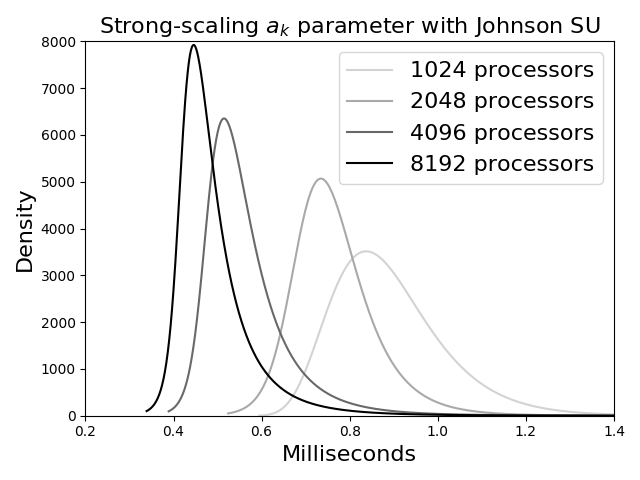
\includegraphics[width=6cm]{../plots/GMRES_ex48_1000000_a_k_strong_scaling_johnsonsu.png}
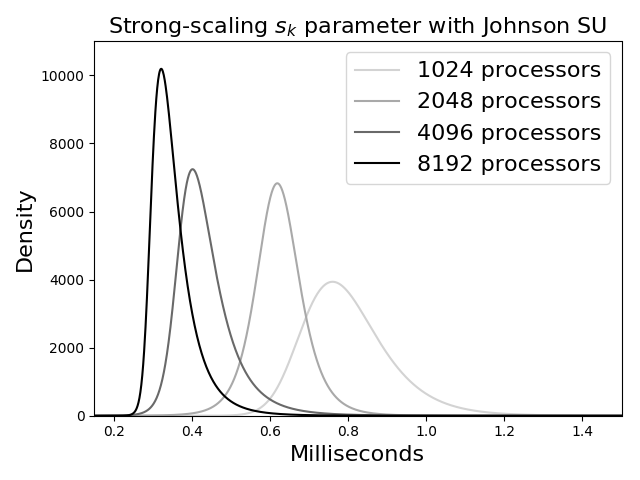
\includegraphics[width=6cm]{../plots/PGMRES_ex48_1000000_s_k_strong_scaling_johnsonsu.png} 
\caption{GMRES ex48 strong-scaling results on $P = 1024 - 8192$ processors.} \label{fig:strong-scaling}
\end{figure}
 
\begin{figure}[b]
\centering
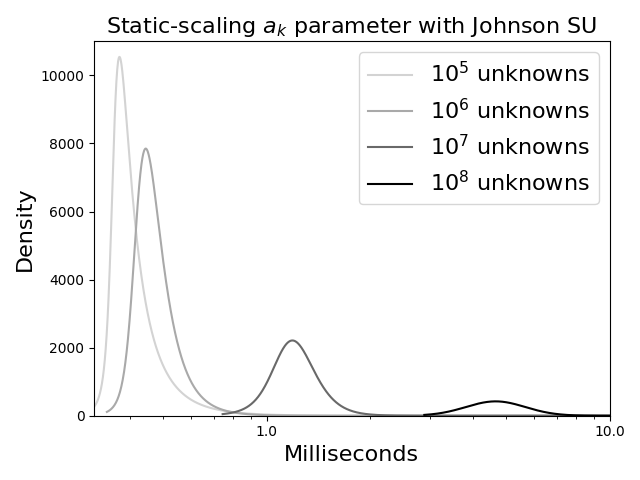
\includegraphics[width=6cm]{../plots/GMRES_ex48_1000000_a_k_static_scaling_johnsonsu.png}
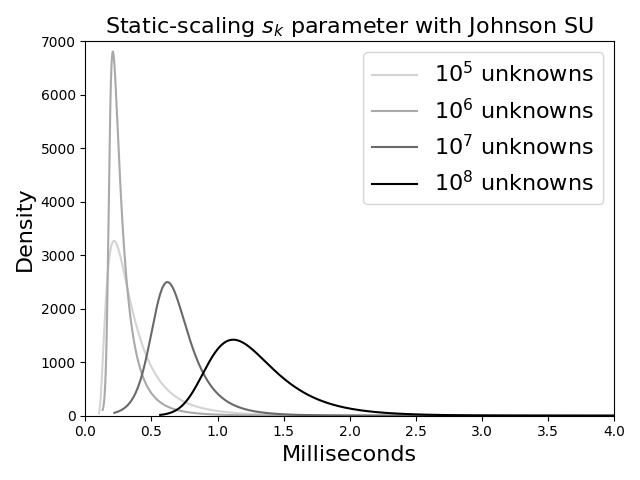
\includegraphics[width=6cm]{../plots/PGMRES_ex48_1000000_s_k_static_scaling_johnsonsu.png} 
\caption{GMRES ex48 static-scaling results for $10^5 - 10^8$ unknowns.} \label{fig:static-scaling}
\end{figure}

With strong-scaling experiments, we see how varying the processor count affects Krylov method performance for a fixed problem. We repeat runs of ex48 with  $10^6$ unknowns on $P = 1024 - 8192$ processors. 
We see that, for a fixed number of unknowns, as we decrease problem size the Johnson SU distribution shifts to the right and spreads out for both uniform parameters since each processor does more work and is more likely to experience a detour. 
Similarly, we perform static-scaling results where we keep the number of processors fixed at $P=8192$ and vary the number of unknowns to see the effect of computation on underlying iteration distributions.
Static-scaling changes exaggerate what we see for strong-scaling.

%Pipelined methods have the potential to outperform than traditional Krylov methods when enough processors are deployed so that communication dominates the algorithm, since pipelined methods can overlap computation with communication. We found that on 8192 processors with $10^6$ unknowns, PGMRES outperforms GMRES for PETSc tutorials ex23 and ex48. The pipelined limit is reached, however, closer to $10^7$ unknowns on 8192 processors, when computation dominates each iteration.

\subsection{BCGS}\label{sec:bcgs}

We solve PETSc ex23, the one-dimensional Laplacian problem, using the Stabilized Biconjugate Gradient method (BCGS) and a pipelined version (PIPEBCGS) with 5000 linear iterations and $10^6$ unknowns on Theta.  

Many aspects of the BCGS and PIPEBCGS computations are consistent with GMRES and PGMRES, such as non-stationary iterates and nearly constant BCGS runtimes on a given node of Theta. 
Figure \ref{fig:bcgs} shows uniform parameter $a_k$ and $s_k$ histograms with GMRES and PGMRES for comparison. 
Although with different parameters, the BCGS and PIPEBCGS distributions look like they can be modeled by Johnson SU distribution family, 
suggesting that our performance model is applicable to Krylov methods outside of GMRES methods.
GMRES and PGMRES outperform BCGS and PIPEBCGS and have quicker minimum iteration times (Johnson SU distributions shifted to the left for uniform parameter $a_k$), but runtimes are  tightly grouped.
Performance results for BCGS and PIPEBCGS using our non-stationary stochastic models are in shown Table \ref{tab:performance-model-2}.


\begin{figure}[t]
\centering
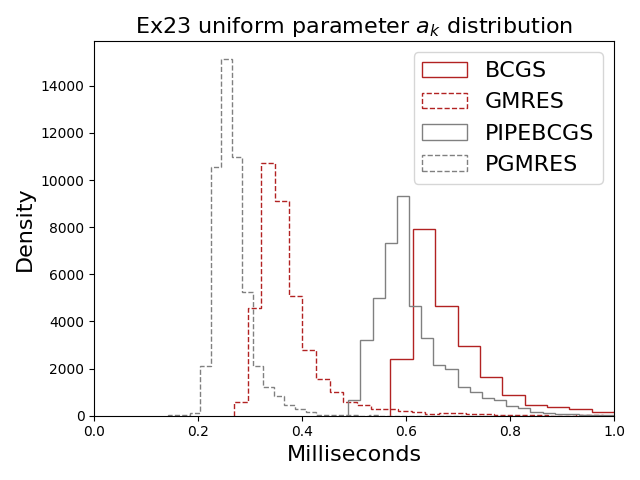
\includegraphics[width=6cm]{../plots/BCGS_GMRES_PIPEBCGS_PGMRES_ex23_8192_1000000_uniform_a_k.png} 
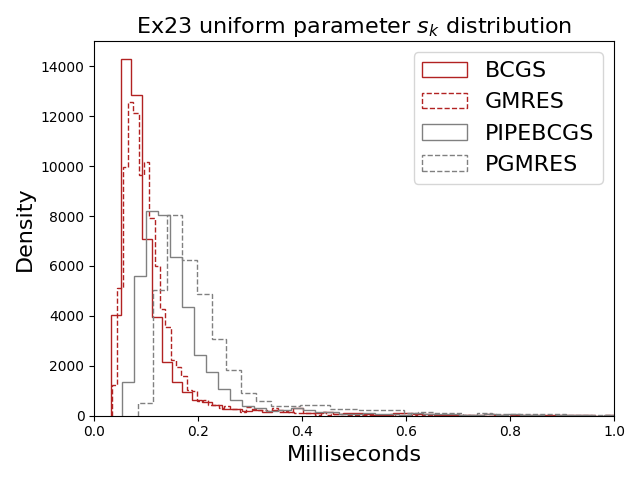
\includegraphics[width=6cm]{../plots/BCGS_GMRES_PIPEBCGS_PGMRES_ex23_8192_1000000_uniform_s_k.png}
\caption{BCGS and PIPEBCGS uniform parameters compared to GMRES and PGMRES.} \label{fig:bcgs}
\end{figure}

\subsection{Piz Daint}\label{sec:pizdaint}

We repeat experiments on the Cray XC40 Piz Daint supercomputer\footnote{hybrid partition, November 2018} at the Swiss National Computing Center. 
Piz Daint and Theta both employ a Aries Dragonfly interconnect but Piz Daint contains Intel Xeon E5 Haswell  processors \cite{hammarlund2014haswell} on compute nodes, so the differences we see are likely due to different processors or the shared use of a communication network.
Figure \ref{fig:pizdaint} shows runs of ex48 with GMRES and PGMRES on 8192 processors and $10^6$ unknowns. 
In a given iteration, the quickest processor can be much faster on Piz Daint than Theta, but both uniform parameters contain much more variation.
Non-stationary performance model results from Piz Daint are in shown Table \ref{tab:performance-model-2}.

\begin{figure}[b]
\centering
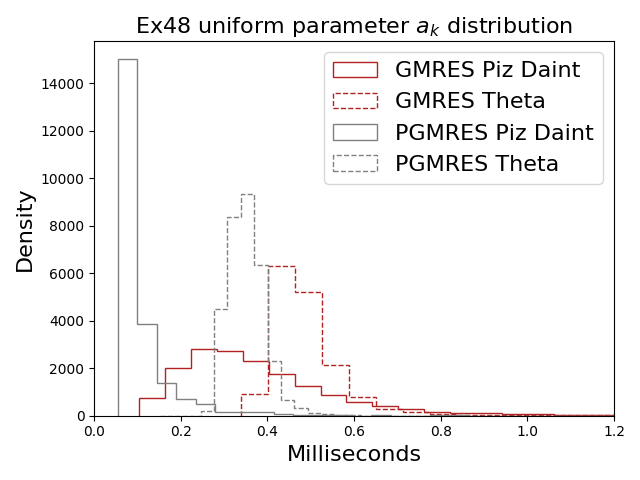
\includegraphics[width=6cm]{../plots/THETA_PIZDAINT_ex48_8192_1000000_uniform_a_k.png} 
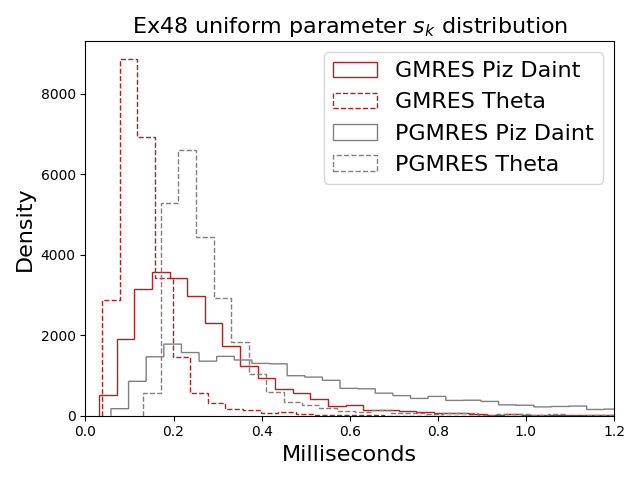
\includegraphics[width=6cm]{../plots/THETA_PIZDAINT_ex48_8192_1000000_uniform_s_k.png}
\caption{GMRES and PGMRES on Theta and Piz Daint.} \label{fig:pizdaint}
\end{figure}


\subsection{Mira}\label{sec:mira}

We repeat ex48 experiments on Mira, an IBM Blue Gene/Q \cite{kumaran2016introduction} at Argonne's ALCF.  
We expect a marked performance difference on Mira since 
nodes on Mira are connected by a 5D Torus Network with hardware to assist collective functions, 
where nodes on Theta are connected by a Cray Aries Network where neighboring workloads share network routes, increasing performance variability \cite{groves2017understanding}. 
Each Blue Gene/Q node also contains a redundant processor that can soak up operating system interrupts, similar to Cray's core specialization feature where one core per node is dedicated to handling OS operations, which reduces core variability \cite{chunduri2017run}.


Figure \ref{fig:mira} shows histograms of iterations from difference places in the GMRES cycle as well as a bulk histogram for all iterations from all processors, which can be thought of as the average performance. Each curve has been normalized to represent a distribution.  
GMRES iterations on Theta at different places in the cycle appear similar to the average. They are noisy enough that our simulation from Section \ref{sec:performance-estimates} provided reasonable results even though we drew uniform parameters $a_k$ and $s_k$ from the same Johnson SU distributions regardless of $k$ in the GMRES cycle. 
With Mira's quiet network, the GMRES iterates are much more distinct suggesting that a refined model that accounts for the amount of work done per iteration would be needed for a priori estimates.
Futhermore, we see a jump in the time between iterations $k \mod 30 = 13$ and $k \mod 30 = 14$ probably due to cache effects and using more storage throughout a GMRES cycle. 
Similar results were found for PGMRES and performance results are in Table \ref{tab:performance-model-2}.




\begin{figure}
\centering
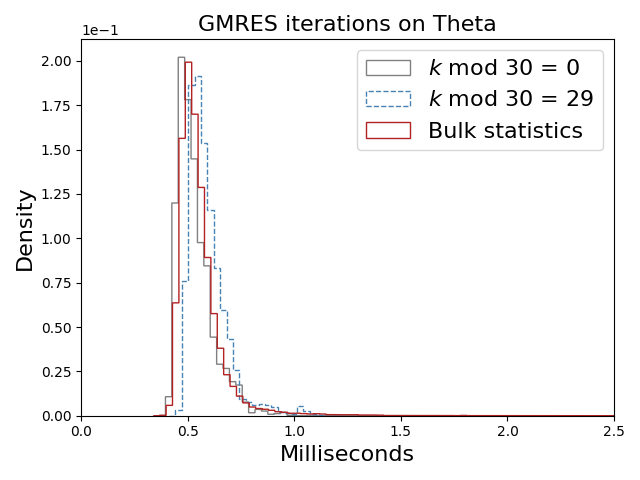
\includegraphics[width=6cm]{../plots/GMRES_ex48_8192_1000000__bulk_statistics_with_k_mod_30_.png}
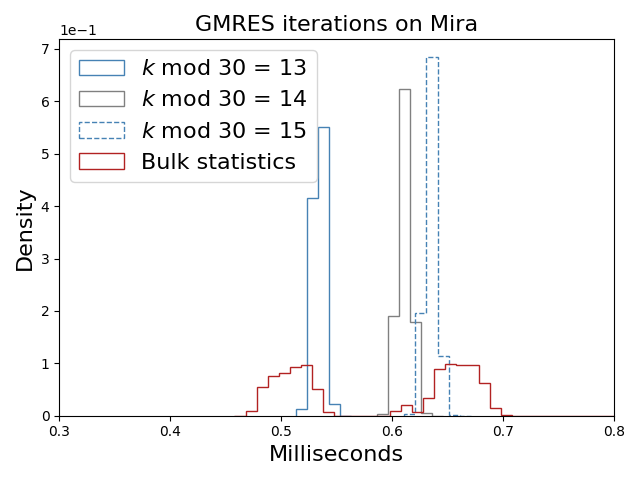
\includegraphics[width=6cm]{../plots/GMRES_MIRA_ex48_8192_1000000__bulk_statistics_with_k_mod_30_.png}
\caption{GMRES ex48 iteration density and Theta and Mira.}  \label{fig:mira}
\end{figure}


\begin{table}[b]
\caption{Non-stationary performance model results for ex23 and ex48 for extended experiments.}
\begin{center}
\begin{tabular}{| l l l | l l } \cline{1-3}
 & \multicolumn{2}{c |}{Theta} & & \\
 ex23 & BCGS & PIPEBCGS & &   \\
KSPSolve & 3.957 & 3.53 & &  \\
 $\widehat{E}_{\text {Unif}}\left[T\right]$ & 4.227 & 3.512 & &  \\ \hline

 & \multicolumn{2}{c |}{Piz Daint} & \multicolumn{2}{c |}{Mira}  \\
 ex48 &  GMRES & PGMRES & GMRES & \multicolumn{1}{c |}{PGMRES} \\
 KSPSolve  & 3.029 & 2.642 & 3.026 & \multicolumn{1}{c |}{2.804} \\
  $\widehat{E}_{\text {Unif}}\left[T\right]$ & 3.541 & 2.473 & 3.189 & \multicolumn{1}{c |}{2.455} \\
\hline  % Please only put a hline at the end of the table
\end{tabular} \label{tab:performance-model-2}
\end{center}
\end{table}


\section{Conclusion and future work} \label{sec:conclusion}

The goal of this work was to gather fine-grained iteration data from runs of Krylov and pipelined Krylov methods to develop a performance model and study the impact of machine interference on these methods. 
We used the data to develop and test stochastic performance models, which are in good agreement with reality. 
Variability during computation suggests that performance is not deterministic and could be better explained in a stochastic setting. 
With descriptive enough statistics we were also able to make a priori performance estimates. 
In future work, nondeterministic performance models can be derived for other parallel algorithms where unpredictable system interference could impact performance.
Insights from performance models can also be used to guide the development of new algorithms, particularly those we expect to be running in less predictable computing environments, such as heavily loaded machines or loosely coupled networks used in cloud computing or those with shared resources.

\iffalse
\section*{Acknowledgements}
Thanks to everyone who offered insight and advice, including Todd Munson, Barry Smith, Ivana Marincic, Vivak Patel, Karl Rupp, and Oana Marin.
\fi

\bibliographystyle{ACM-Reference-Format}
\bibliography{bibli}

\iffalse
\newpage
{\bf Disclaimer.} The submitted manuscript has been created by UChicago Argonne, LLC,
Operator of Argonne National Laboratory (``Argonne'').
Argonne, a U.S. Department of Energy Office of Science laboratory, is
operated under Contract No. DE-AC02-06CH11357. The U.S. Government
retains for itself, and others acting on its behalf, a paid-up
nonexclusive, irrevocable worldwide license in said article to reproduce,
prepare derivative works, distribute copies to the public, and perform
publicly and display publicly, by or on behalf of the Government.
\fi



\end{document}
